\documentclass[10pt, oneside]{memoir}   	% use "amsart" instead of "article" for AMSLaTeX format
\usepackage{geometry}                		% See geometry.pdf to learn the layout options. There are lots.
\geometry{letterpaper}                   		% ... or a4paper or a5paper or ... 
%\geometry{landscape}                		% Activate for rotated page geometry
%\usepackage[parfill]{parskip}    		% Activate to begin paragraphs with an empty line rather than an indent
\usepackage{graphicx}				% Use pdf, png, jpg, or eps§ with pdflatex; use eps in DVI mode

\usepackage{amssymb}
\usepackage[italian]{babel}
%SetFonts
 \usepackage{hyperref}
%SetFonts
\usepackage[utf8]{inputenc}

\title{Finite Fields. Lattice 1}
\author{Valerio Maiolo}
\date{}		
					% Activate to display a given date or no date




\begin{document}
%\section{}
%\subsection{}

\maketitle

\begin{center}
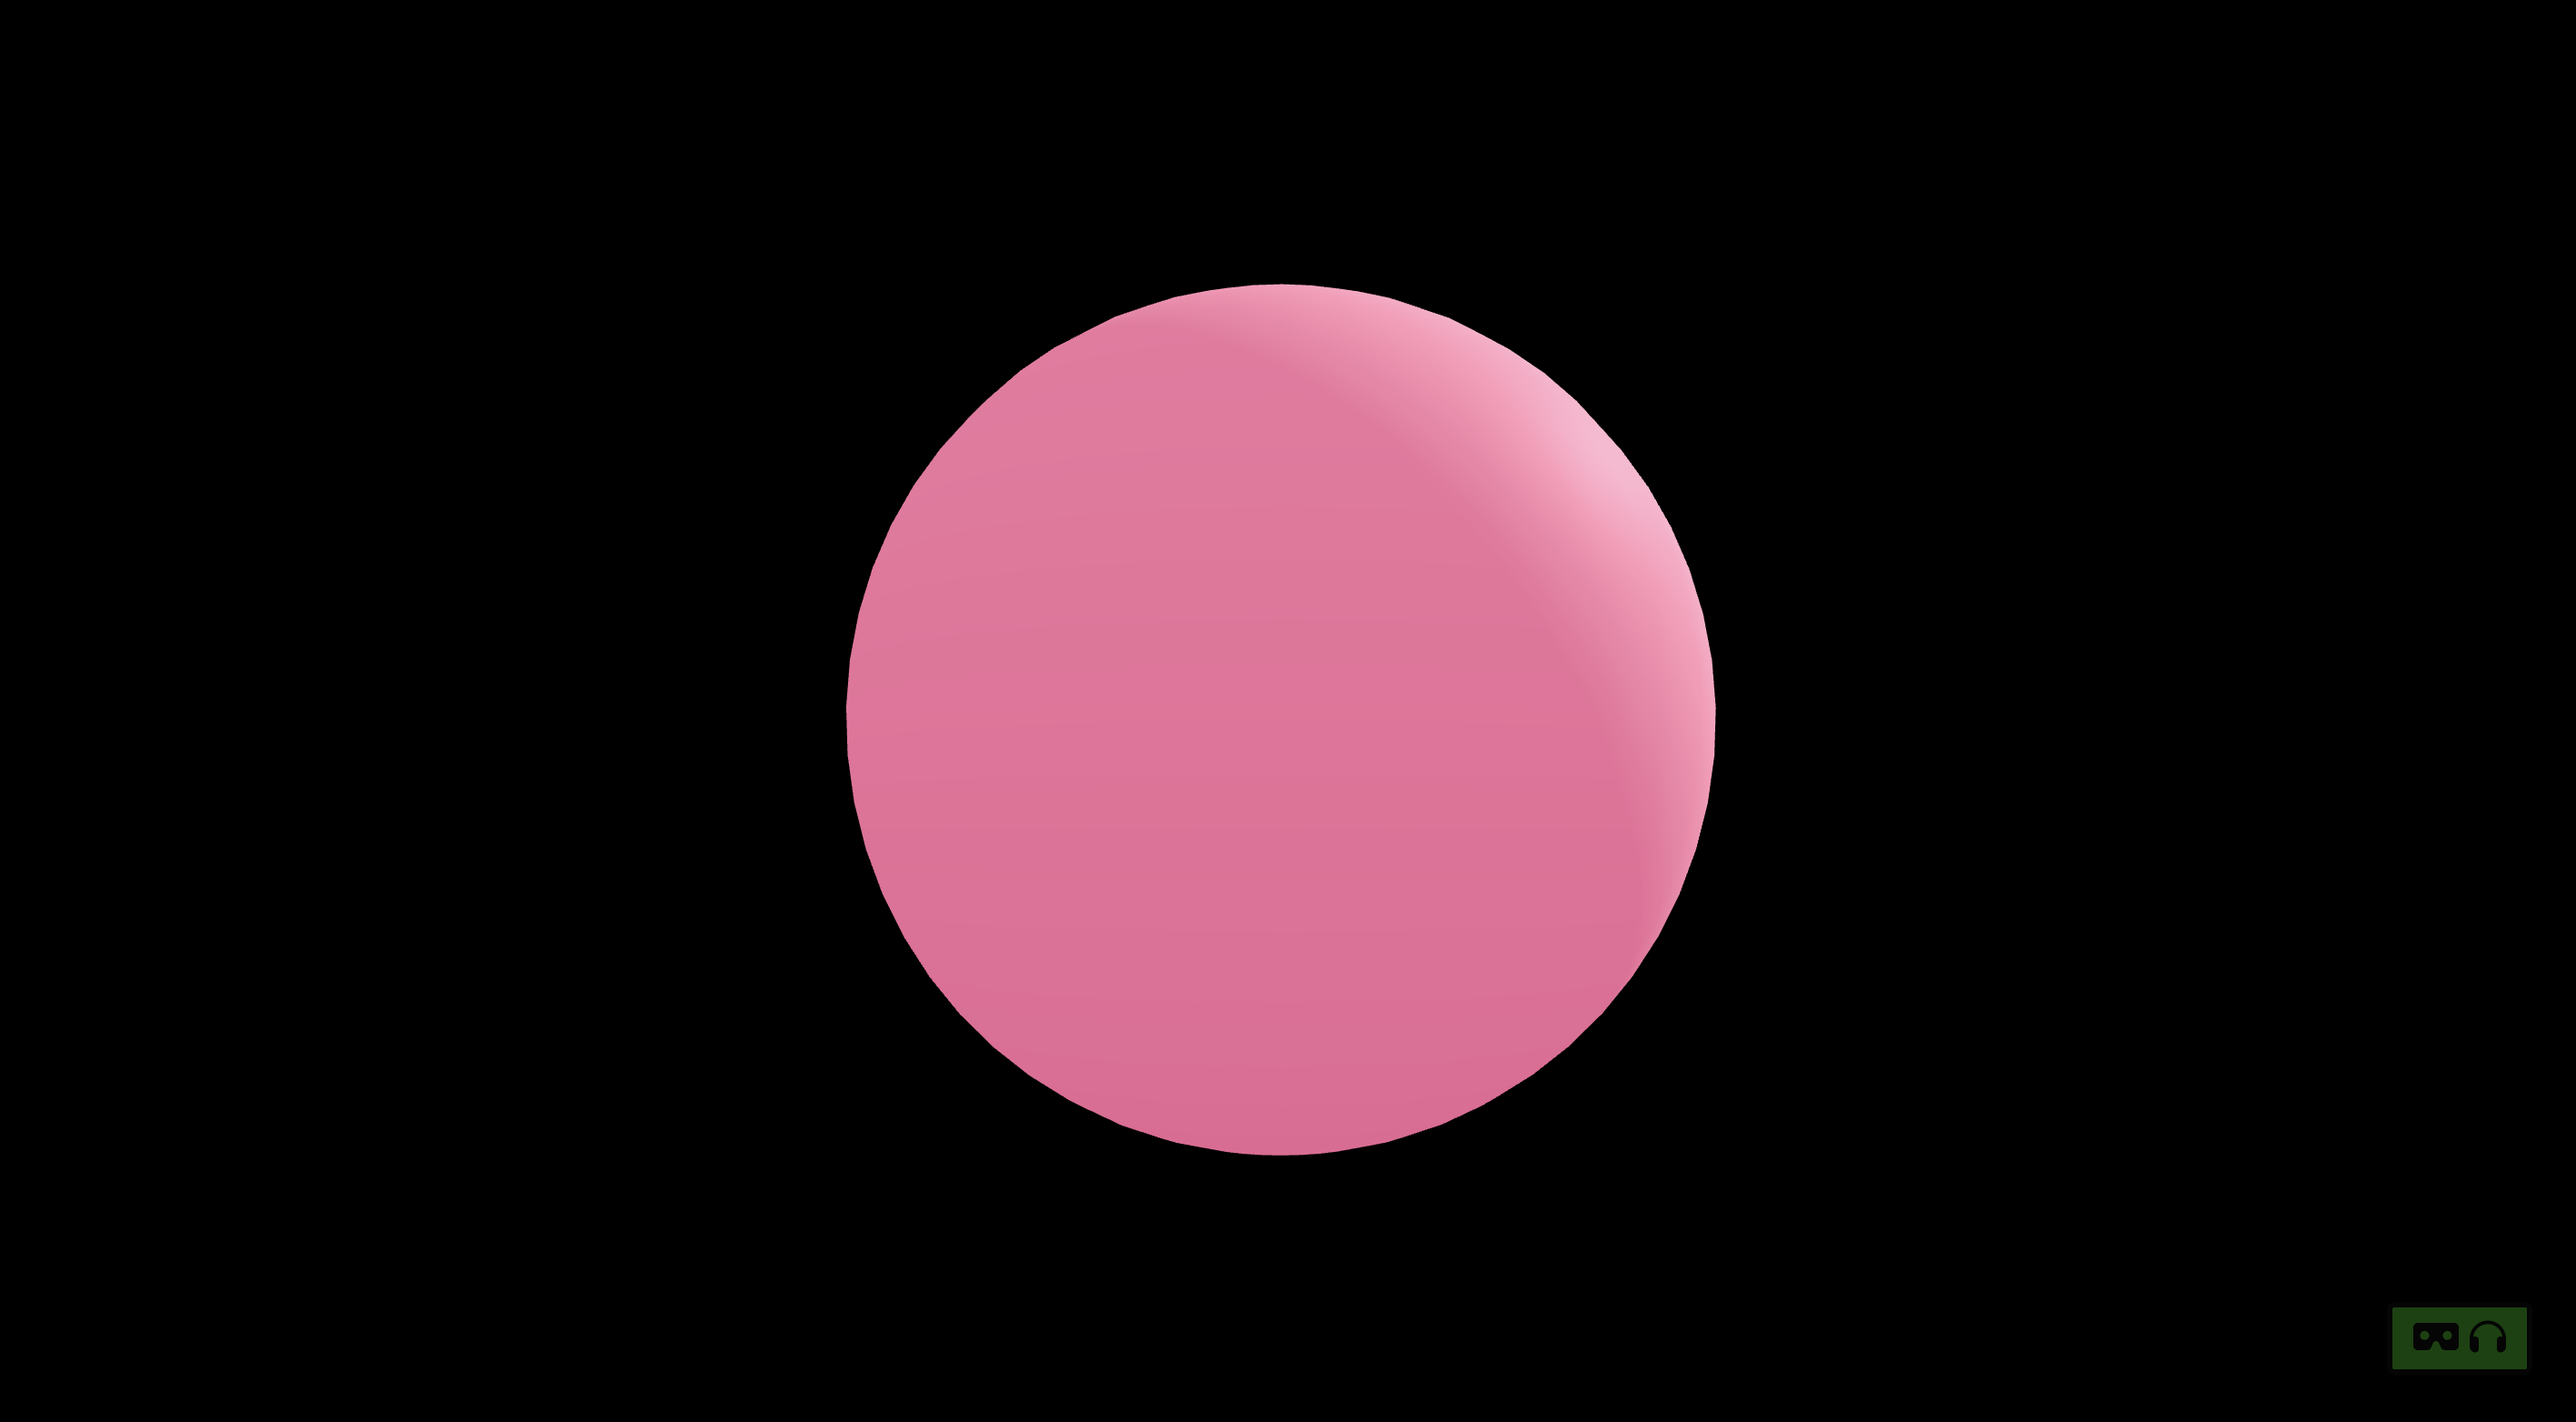
\includegraphics[scale=0.3]{sferaVR.png}
\end{center}

\newpage

\textit{Finite Fields} è il nuovo progetto laboratoriale e transmediale di Valerio Maiolo. In \textit{Finite Fields - Lattice 1}, a partire da un corpus di pratiche fra cui lo studio di sistemi di intonazione naturale, la sintesi del suono programmato con il computer e il canto armonico, Valerio sviluppa una serie di costruzioni cristalline in realtà virtuale che attraverso il movimento rivelano gli aspetti più geometrici del suono. \textit{Finite Fields - Lattice 1} è parte della ricerca di Valerio sulla relazione fra \textit{composizione infinita} e il \textit{medium} con cui essa, necessariamente, deve confrontarsi. L'Internet of Sounds, la realtà virtuale, il browser sono, in questo caso, l'environment designato ad ospitare una composizione in cui ogni istante ha uguale significato e in cui i limiti temporali e spaziali della composizione non possono essere costretti dalla capienza e dai confini del supporto. Nella dissoluzione della dimensione temporale, si dischiude uno spazio interiore in cui l'ascolto diventa un modo attivo di agire, focalizzarsi e muoversi all'interno del corpo sottile del suono, in un'esperienza immersiva e, in ultima analisi, profondamente emotiva. 

\end{document}  